\documentclass[hyperref={colorlinks,citecolor=blue,linkcolor=blue,urlcolor=blue}, aspectratio=1610]{beamer}
\usepackage{xcolor}
\usepackage{pgfpages}
\usepackage[utf8]{inputenc}
\usepackage[english]{babel}
\usepackage{amsmath}
\usepackage{amsmath,amssymb}
\usepackage{tikz}
\usepackage{forest}
\usepackage{qrcode}
\usepackage{graphicx}


\mode<presentation>
{
  \usetheme{Madrid}       % or try default, Darmstadt, Warsaw, ...
  \usecolortheme{beaver} % or try albatross, beaver, crane, ...
  \usefonttheme{structurebold}    % or try default, structurebold, ...
  \setbeamertemplate{navigation symbols}{}
  \setbeamertemplate{caption}[numbered]
} 



\definecolor{codegreen}{rgb}{0,0.6,0}
\definecolor{codegray}{rgb}{0.5,0.5,0.5}
\definecolor{codepurple}{rgb}{0.58,0,0.82}
\definecolor{backcolour}{rgb}{0.95,0.95,0.92}

\usepackage{listings}
\lstdefinestyle{mystyle}{
    commentstyle=\color{codegreen},
    keywordstyle=\color{blue},
    stringstyle=\color{codepurple},
    basicstyle=\ttfamily\small,
    breakatwhitespace=false,
    breaklines=true,
    captionpos=b,
    keepspaces=true,
    showspaces=false,
    showstringspaces=false,
    showtabs=false,
    tabsize=2
}

% \pgfpagesuselayout{resize to}[%
%   physical paper width=8in, physical paper height=6in]

\title[IbraFSG 8: The Final Week]{IbraFSG\texttrademark{} 8 - Week 12; Algorithms and Efficiency}


\author{Ibrahim Chehab}
\institute{UTM RGASC}
\date{\today}

\begin{document}

\begin{frame}
  \titlepage
\end{frame}

\begin{frame}{Table of Contents}
  \tableofcontents
\end{frame}

\section{Introduction}

\subsection{FSG HouseKeeping}
\begin{frame}
  \frametitle{FSG HouseKeeping}
  \begin{enumerate}
    \item \textbf{Reminder that a new FSG Session has been added:}
    \begin{itemize}
      \item \textbf{When?} \textit{Fridays, 12:00-1:00PM}
      \item \textbf{Where?} \textit{IB210}
    \end{itemize}
    \pause
    \item \textbf{Assignment 2 Deadline Coming Up!} Assignment 2 is due today at 5:00PM! Don't forget to submit it on MarkUs!
    \pause
    \item \textbf{New Study Session Drop Ins!} \\ Feeling Stressed about exams? Don't know where to start? Drop by the MN3260 for a study skills session! 
    \begin{itemize}
      \item \textbf{When:} April $3^{rd}$ 1-2PM
      \item \textbf{Where:} MN3260
    \end{itemize}
    \pause
    \item \textbf{Join the UTM CS Discord Server!} \url{https://discord.gg/utmcs}
    \begin{itemize}
      \item \textbf{Note:} The server is not affiliated with the RGASC, CSC148H5, or the University of Toronto Mississauga
    \end{itemize}
    \pause
    \item \textbf{MEGA FSG Coming Soon!} Stay tuned for a MEGA FSG session to help you prepare for the final exam!
  \end{enumerate}

\end{frame}

\subsection{Welcome back to IbraFSGs\texttrademark{}}
\begin{frame}
    \frametitle{Welcome back to IbraFSGs\texttrademark{}}
    \begin{itemize}
        \item Welcome back to IbraFSGs\texttrademark{}! Hello to new people and welcome back to tenured members.
        \item This week we will be going over algorithms and complexity analysis
        \item Todays session will act as a prelude to \textit{CSC236}
        \begin{itemize}
          \item \textit{CSC236} is the course where you will learn about the theory of computation
          \item The entire course has a backbone of \textit{induction} and \textit{recursion}
          \item Towards the end of the course, you will learn about DFAs, NFAs, and Turing Machines (i.e: a DFA is a quintuple $(Q, \Sigma, \delta, q_0, F)$)
        \end{itemize}
        \pause
        \item \url{https://www.bigocheatsheet.com/}
        \pause
        \item \textbf{Fun Fact:} In \textit{CSC263}, you will use something called the \textit{Master Theorem} to analyze the complexity of divide and conquer algorithms like \textit{MergeSort} and \textit{QuickSort}
    \end{itemize}  

\end{frame}

\begin{frame}
  \frametitle{Bonus! The Master Theorem: A Comprehensive Overview}
  \textbf{NOTE: THIS IS COMPLETELY OUT OF SCOPE FOR CSC148! JUST HERE FOR FUN FACT!!}
  \textbf{The Master Theorem provides a method for solving recurrence relations of the form:}
  \begin{align*}
    T(n) = aT\left(\frac{n}{b}\right) + f(n)
  \end{align*}
  where, 
  \begin{itemize}
    \item $a \geq 1$ and $b > 1$ are constants,
    \item $f(n)$ is an asymptotically positive function.
  \end{itemize}
  
  \textbf{The theorem is divided into three cases:}
  \begin{enumerate}
    \item \textbf{Case 1:} If $f(n) \in O(n^{\log_b a - \varepsilon})$ for some $\varepsilon > 0$, then $T(n) \in \Theta(n^{\log_b a})$.
    \item \textbf{Case 2:} If $f(n) \in \Theta(n^{\log_b a}\log^k n)$ for some $k \geq 0$, then $T(n) \in \Theta(n^{\log_b a}\log^{k+1} n)$.
    \item \textbf{Case 3:} If $f(n) \in \Omega(n^{\log_b a + \varepsilon})$ for some $\varepsilon > 0$, and if $af\left(\frac{n}{b}\right) \leq cf(n)$ for some $c < 1$ and sufficiently large $n$, then $T(n) \in \Theta(f(n))$.
  \end{enumerate}

  \begin{center}
    \textit{Tl;Dr - CS isn't all about coding, there's a lot of math involved too!}\\
    \textit{Tldrdr - CS gets real hard real fast}      
  \end{center}
\end{frame}


\subsection{A Recap of the UltraSheet\texttrademark{}}
\begin{frame}{A Recap of the UltraSheet\texttrademark{}}
  \begin{itemize}
    \item An \textit{UltraSheet\texttrademark{}} is a "cheat sheet" that you compile for \textbf{yourself} to review course materials 
    \begin{itemize}
      \item Sharing UltraSheets\texttrademark{} is \textbf{counter-productive} and \textbf{will not help you learn the material}
      \item However, reviewing content in a group and simultaneously updating your UltraSheets\texttrademark{} is a good idea
    \end{itemize}
    \item It acts like your own personalized textbook chapter
    \begin{itemize}
      \item It allows you to \textbf{regurgitate all the course information in a contiguous, organized manner} and helps you \textbf{find gaps in your knowledge}
      \item You should \textbf{not} be copying the textbook or lecture slides verbatim; You should be \textbf{summarizing} the content in your own words while tying in examples and analogies
    \end{itemize}
    \item UltraSheets\texttrademark{} help with type 1 and 2 questions 
  \item In case you didn't notice yet, Petersen \textit{loves Type 1} and \textit{Type 2} questions - Use this information how you will ;P
  \end{itemize}

\end{frame}

\section{Algorithms and Efficiency}

\subsection{Key Terms}

\begin{frame}{Key Terms}
  \textbf{Required Key Terms:} The following key terms are required for this week's content. You should be able to define and explain these terms in your UltraSheets\texttrademark{}:
    \begin{itemize} 

      \item \textbf{Big-O Notation ($\mathcal{O}(n)$)}
      \begin{itemize}
        \item Upper Bound
        \item A function $f(n)$ is $\mathcal{O}(g(n))$ if there exists a constant $c > 0$ and $n_0 > 0$ such that $f(n) \leq c \cdot g(n)$ for all $n \geq n_0$
      \end{itemize}
      \pause
      \item \textbf{Big-Theta Notation ($\Theta(n)$)}
      \begin{itemize}
        \item Tight Bound
        \item A function $f(n)$ is $\Theta(g(n))$ if and only if $f(n)$ is $\mathcal{O}(g(n))$ and $f(n)$ is $\Omega(g(n))$
        \item In other words; $f(n)$ is $\Theta(g(n))$ if and only if there exist constants $c_1 > 0$, $c_2 > 0$, and $n_0 > 0$ such that $c_1 \cdot g(n) \leq f(n) \leq c_2 \cdot g(n)$ for all $n \geq n_0$
        
      \end{itemize}
    \end{itemize}    
\end{frame}

\begin{frame}{Key Terms (Cont'd)}
  \textbf{Suggested Key Terms:} The following key terms are \textit{recommended} for further studying this week's content. Most are out of the scope of the course and are \textbf{not} required. 
  \begin{itemize} 
    \item \textbf{Big-Omega Notation ($\Omega(n)$)}
    \begin{itemize}
      \item Lower Bound
      \item A function $f(n)$ is $\Omega(g(n))$ if there exists a constant $c > 0$ and $n_0 > 0$ such that $f(n) \geq c \cdot g(n)$ for all $n \geq n_0$
    \end{itemize}
    \item \textbf{The Master Theorem}
    \begin{itemize}
      \item A method for solving recurrence relations of the form $T(n) = aT\left(\frac{n}{b}\right) + f(n)$
      \item Allows for finding time complexity of divide and conquer algorithms
    \end{itemize}
    \item \textbf{Induction (Weak, Strong, Structural)}
    \begin{itemize}
      \item Recall this from MAT102
      \item Used to formally prove the correctness and efficiency-class of algorithms
    \end{itemize}
    Aaaaand.... that's it for today! 
  \end{itemize}
\end{frame}

\begin{frame}
  \frametitle{Example of CSC236 Problem (1/3):}
  \textbf{Question 1:} Show that if $f \in \mathcal{O}(g)$ and $g \in \Theta(h)$, then $f + g \in \Theta(h)$.

  \begin{proof}
    Given $f \in \mathcal{O}(g)$, there exists $c_1, n_0 > 0$ such that $f(n) \leq c_1g(n)$ for all $n \geq n_0$. For $g \in \Theta(h)$, there are constants $c_2, c_3, n_1 > 0$ making $c_2h(n) \leq g(n) \leq c_3h(n)$ for all $n \geq n_1$.

    We aim to find $c_4, c_5, n_2 > 0$ satisfying $c_4h(n) \leq f(n) + g(n) \leq c_5h(n)$ for all $n \geq n_2$.

    Combining our initial conditions, we get:
    \begin{align*}
        0 \leq f(n) \leq c_1g(n) \\
        c_2h(n) \leq g(n) \leq c_3h(n)
    \end{align*}
  \end{proof}
\end{frame}

\begin{frame}
  \frametitle{Example of CSC236 Problem (2/3):}
  \textbf{Continuation of Proof:}

  \begin{proof}[Proof (continued)]
    Combining the given, for $n \geq \max(n_0, n_1)$:
    \begin{align*}
      c_2h(n) \leq f(n) + g(n) \leq c_1g(n) + c_3h(n)\\
    \end{align*}
    \pause
    From the definition of $\Theta(n)$, we know that $g(n)$ is upper-bounded by $c_3 \cdot h(n)$ for all $n \geq n_1$. Hence, we can simplify the above inequality to:
    \begin{align*}
        \implies c_2 \cdot h(n) \leq f(n) + g(n) \leq c_1 \cdot \left(c_3 \cdot h(n)\right) + c_3 \cdot h(n) \quad \text{for all } n \geq \max(n_0, n_1) \\
    \end{align*}
    \vspace*{-1em}
    \pause
    Factoring out $h(n)$ from the RHS, we get:
    \begin{align*}
      \implies c_2 \cdot h(n) \leq f(n) + g(n) \leq (c_1 \cdot c_3 + 1) \cdot h(n) \quad \text{for all } n \geq \max(n_0, n_1)
    \end{align*}
    \vspace*{-1em}
  \end{proof}
\end{frame}

\begin{frame}
  \frametitle{Example of CSC236 Problem (3/3):}
  \textbf{Finishing off the Proof:}

  \begin{proof}[Proof (continued)]
    \begin{align*}
      \implies c_2 \cdot h(n) \leq f(n) + g(n) \leq (c_1 \cdot c_3 + 1) \cdot h(n) \quad \text{for all } n \geq \max(n_0, n_1)
    \end{align*}

    Take $c_4 = c_2$ and $c_5 = c_1 \cdot c_3 + 1$. We have shown that $f(n) + g(n)$ is upper-bounded by $(c_1 \cdot c_3 + 1) \cdot h(n)$ for all $n \geq \max(n_0, n_1)$. We can also show that $f(n) + g(n)$ is lower-bounded by $c_2 \cdot h(n)$ for all $n \geq \max(n_0, n_1)$.

    Hence, we have shown that $f(n) + g(n) \in \Theta(h(n))$, thus completing the proof.
  \end{proof}
  \textit{Note: This proof is a bit more advanced than what you would see in CSC148. It's meant to give you a taste of what you'll see in CSC236.}\\
  \textit{Note 2: This proof has been heavily condensed for time purposes. The actual proof would be more detailed and rigorous.}
\end{frame}

\section{Practice Problems}

\begin{frame}
  \frametitle{Jamboard Link}
  \begin{center}
    \qrcode[height=2in]{https://jamboard.google.com/d/1kl17umPnvJRR505O3BZTfCjjE-XjC9VcbP-Z2Mh7CwM/edit?usp=sharing}\\
    \url{https://tinyurl.com/ibrafsg0403}\\
    \textit{0403 for April $3^{rd}$}\\
    \textbf{Note:} Jamboard isn't ideal because of its limitations, hence I'm working on my own alternative. Stay tuned!
  \end{center}
\end{frame}

\subsection{Practice Problem I: The Tightest Bound} 
\begin{frame}[fragile]
  \frametitle{Practice Problem I: The Tightest Bound}
  Peace and d.aki are arguing over the tightest upper-bound for the following function. Peace argues that it's $\mathcal{O}(n^2)$ while d.aki argues that it's $\mathcal{O}(n^3)$. Given the following function, who is correct? Justify your answer.

  \begin{lstlisting}[language=Python,style=mystyle]
def mystery(n: int):
  L = []
  for i in range(n):
      for j in range(min(50, n)):
          L.insert(0, j)
  \end{lstlisting}

  \textit{Hint: Recall the definition of $\mathcal{O}$ notation}\\
  \textit{Hint 2: Consider modeling a piecewise function $T(n)$ dictating the number of steps taken by the function for arbitrary input $n$}\\
  \onslide<2->{
    Recall:
    For a function $f$ to be an element of $\mathcal{O}(g)$, there must exist constants $c > 0$ and $n_0 > 0$ such that $f(n) \leq c \cdot g(n)$ for all $n \geq n_0$
  }
\end{frame}

\begin{frame}[fragile]
  
  \frametitle{Practice Problem I Debrief}
  What if we changed the \texttt{min} to \texttt{max}? Abdulkader thinks it's still $\mathcal{O}(n^2)$, but drew thinks it's $\mathcal{O}(n^3)$. Who is correct. Justify your answer.
  \begin{lstlisting}[language=Python,style=mystyle]
def mystery2(n: int):
  L = []
  for i in range(n):
      for j in range(max(50, n)):
          L.insert(0, j)
  \end{lstlisting}
  \textit{Hint: Modify your piecewise function $T(n)$ to account for the change in the function, then compare the two functions.}\\
\end{frame}
\subsection{Practice Problem II: FindMiiComplexity}
\begin{frame}[fragile]
  \frametitle{Practice Problem II: FindMiiComplexity}
  What is the worst-case asymptotic complexity of the following function? Justify your answer.
  \begin{lstlisting}[language=Python,style=mystyle]
def foo(x: int):
  n = x
    for i in range(n):
      if n <= 50:
        for j in range(n):
          x += 1
      if n <= 100:
        for j in range(n):
          if n <= 75:
            for k in range(n):
              x += 1
  \end{lstlisting}
  \textit{Hint: Split each part of the function into its own piecewise function $T(n)$, then combine them to find the overall complexity.}\\
  \textit{Hint 2: This problem is probably harder than anything you'll ever get in CSC148}\\
  \onslide<2->{
    \textbf{Bonus (time permitting):} Change one line of this function to make it $\mathcal{O}(n)$
  }
\end{frame}

\section{Conclusion}

\subsection{A Final Challenge\dots}
\begin{frame}
  \frametitle{A Final Challenge...}
  The following question is definitely a \textit{CSC236}-level problem, and you will NOT be tested on it in CSC148 - I REPEAT: \textbf{YOU WILL NOT BE TESTED ON THIS IN CSC148}. However, it's a fun problem to think about and will give you a taste of what you'll see in \textit{CSC236}.\\
\end{frame}

\subsection{Goodbye, for now...}

\begin{frame}
  \frametitle{Thank you for coming!}
  \centering
  \begin{figure}
    
\includegraphics[width=0.5\textwidth]{that's_all_folks.jpeg}
    \caption{Image courtsey of Looney Tunes\texttrademark{} and Warner Bros.\texttrademark{}}
  \end{figure}
\end{frame}

\begin{frame}
  \frametitle{Thank you for coming!}
  \centering
  \begin{figure}
    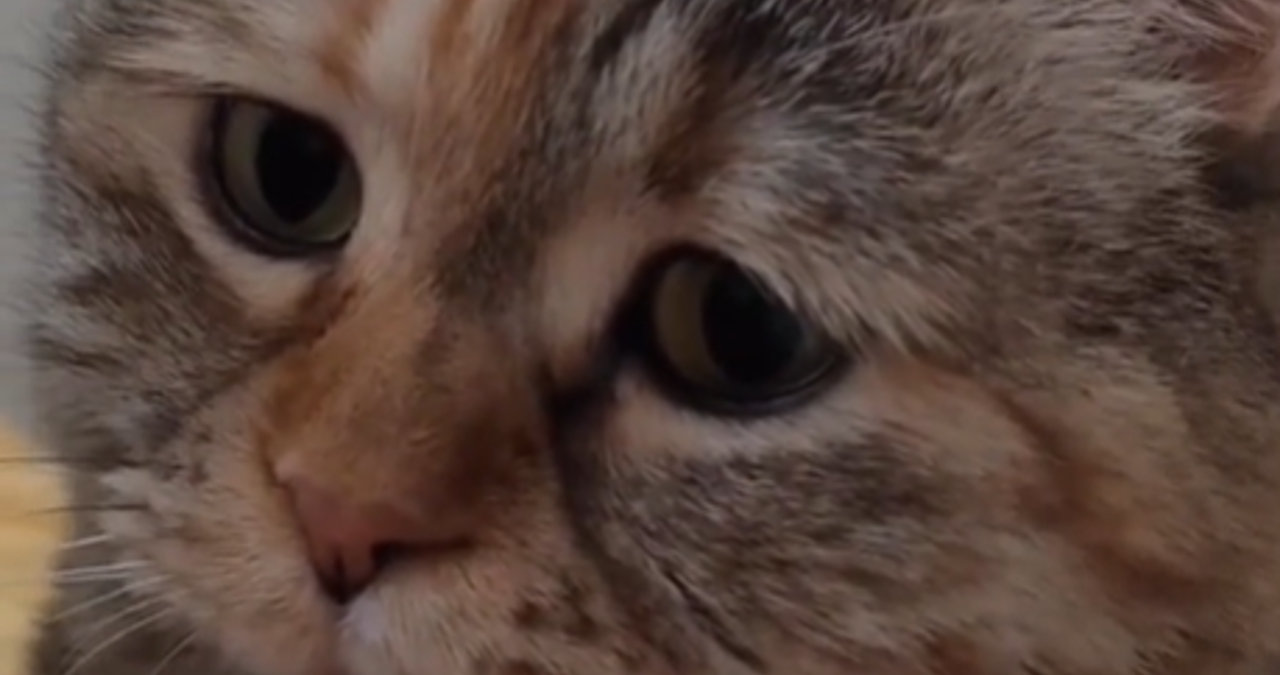
\includegraphics[width=0.5\textwidth]{sadcatcover.jpg}
    \caption{Ibrahim right now because FSGs are over}
  \end{figure}
  Genuinely, thank you for coming to my FSGs. If anything, I hope I made CSC148 easier for you. This has truly been an amazing experience for me, and I hope to see you all in the future (potentially as a TA :eyes:)
  Feel free to reach out to me on Discord or on the UTM CS Discord server if you have any questions or need help with anything.\\

  \textbf{In all seriousness, keep an eye out for our MEGA FSG coming soon....}
\end{frame}

\end{document}